\documentclass[12pt,a4paper]{article}

\usepackage[utf8]{inputenc}
\usepackage[french]{babel}
\usepackage{alphabeta}
\usepackage{ragged2e}

\usepackage[pdftex]{graphicx}
\usepackage[top=1in, bottom=1in, left=1in, right=1in]{geometry}

\linespread{1.06}
\setlength{\parskip}{8pt plus2pt minus2pt}

\widowpenalty 10000
\clubpenalty 10000

\newcommand{\eat}[1]{}
\newcommand{\HRule}{\rule{\linewidth}{0.5mm}}

\usepackage[official]{eurosym}
\usepackage{enumitem}
\setlist{nolistsep,noitemsep}
\usepackage[hidelinks]{hyperref}
\usepackage{cite}
\usepackage{lipsum}


\begin{document}
    \renewcommand{\abstractname}{Un résume}
    \renewcommand{\contentsname}{Table des matières}
    \renewcommand{\refname}{Table de références}

%===========================================================
    \begin{titlepage}
        \begin{center}

% Top 
            
\includegraphics[width=0.55\textwidth]{universite_Montpellier_.jpg}~\\[2cm]


% Title
            \HRule \\[0.4cm]
            { \LARGE
            \textbf{Rapport de - HMIN234 Web Sémantique -}\\[0.4cm]
            \emph{TP2 - Web Sémantique et Social : Interrogation de données RDF}\\[0.4cm]
            }
            \HRule \\[1.5cm]


% Author
            { \large
            22008346 ADOLPHE Benjamin  \\[0.1cm]
            22014998 LAAROUSSI Laila\\[0.1cm]
            \texttt{M1 DECOL}
            }

            \vfill

%\textsc{\Large Cyprus University of Technology}\\[0.4cm]
            \textsc{\large Université de Montpellier - Faculté des Sciences}\\[0.4cm]


% Bottom
            {\large \selectlanguage{french}\today}

        \end{center}
    \end{titlepage}
    \newpage
    \setcounter{page}{1}

%===========================================================
%===========================================================


    \section{Le graphe des Participants à l'UE Web Sémantique et Social:}
    \justify{
        Voir le fichier Exo1.ttl.
    }


    \section{SPARQL : Interrogation et méta-interrogation :}
    \begin{justify}
        Mod\`ele : Voir dans le dossier SPARQL src/main/java/Movies.java
        \begin{enumerate}
            \item \underline{S\'eparer les triplets contenant des connaissances ontologiques des triplets repr\'esentant} \underline{des donn\'ees.}
            \begin{verbatim}
    @prefix movies: <http://www.lirmm.fr/ulliana/movies#> .
    @prefix rdfs: <http://www.w3.org/2000/01/rdf-schema#> .
    @prefix rdf: <http://www.w3.org/1999/02/22-rdf-syntax-ns#> .
    @prefix owl: <http://www.w3.org/2002/07/owl#> .
    @prefix dbp: <http://dbpedia.org/> .

    movies:directedBy rdfs:domain movies:Movie .
    movies:playsIn rdfs:domain movies:Actor .
    movies:playsIn rdfs:range movies:Movie .
    movies:Actor rdfs:subClassOf movies:Artist .
    movies:Director rdfs:subClassOf movies:Artist .
    movies:Director rdfs:subClassOf movies:Artist .
    movies:title rdf:type owl:DataTypeProperty .
    movies:title rdfs:domain movies:Movie .

    //Données
    movies:m2 movies:title "Vertigo" .
    movies:m1 rdf:type movies:Movie .
    movies:m3 movies:directedBy dbp:Alfred_Hitchcock .
    movies:a1 movies:playsIn movies:m4 .
            \end{verbatim}
            \item \underline{Donner la requ\^ete SPARQL qui s\'electionne tous les (identifiants des) films.} \\
            \begin{verbatim}
String q2_1 = "PREFIX rdf: <http://www.w3.org/1999/02/22-rdf-syntax-ns#> "
                    + "PREFIX mov: <http://www.lirmm.fr/ulliana/movies#> "
                    + "SELECT ?s "
                    + "WHERE {?s rdf:type mov:Movie}";
            \end{verbatim}
            \item \underline{Donner la requ\^ete SPARQL qui s\'electionne toutes les sous-classes de la classe artiste.}\\
            \begin{verbatim}
String q2_2 ="PREFIX rdf: <http://www.w3.org/1999/02/22-rdf-syntax-ns#> "
                + "PREFIX mov: <http://www.lirmm.fr/ulliana/movies#> "
                + "SELECT ?movies "
                + "WHERE{{ ?movies rdf:type mov:Movie .  }"
                + "  UNION { ?movies mov:title ?x . }"
                + "  UNION { ?movies mov:directedBy ?x . }"
                + "  UNION { ?x mov:playsIn ?movies . }}";
            \end{verbatim}
            \item \underline{Donner la requ\^ete SPARQL qui s\'electionne tous les acteurs}
            \begin{verbatim}
String q2_3 = "PREFIX rdfs: <http://www.w3.org/2000/01/rdf-schema#> "
                + "PREFIX mov: <http://www.lirmm.fr/ulliana/movies#> "
                + "SELECT ?s "
                + "WHERE {?s rdfs:subClassOf mov:Artist}";
            \end{verbatim}
            \item \underline{Pour chaque requ\^ete, dire s\rq{il} s\rq{agit} d\rq{une} interrogation ou d\rq{une} m\'eta-interrogation}
            \begin{itemize}
                \item Q\_1 : interrogation
                \item Q\_2 : interrogation
                \item Q\_3 : m\'eta-interrogation
            \end{itemize}
        \end{enumerate}
    \end{justify}


    \section{L'exploration d'un endpoint SPARQL: le cas DBPedia: }
    \begin{justify}
        \begin{enumerate}
            \item \underline{Choisissez une classes de l\rq{ontologie} qui commence par la premi\`ere lettre de votre nom,} \underline{et donnez la liste de
            ses sous-classes.} \\
            \begin{verbatim}
PREFIX rdf: <http://www.w3.org/1999/02/22-rdf-syntax-ns#>
PREFIX owl: <http://www.w3.org/2002/07/owl#>
SELECT ?subclass
WHERE {
?subclass rdfs:subClassOf ?varClass .
FILTER regex(?varClass, "http://dbpedia.org/ontology/SportsLeague").
}
LIMIT 100
            \end{verbatim}
            \begin{center}
                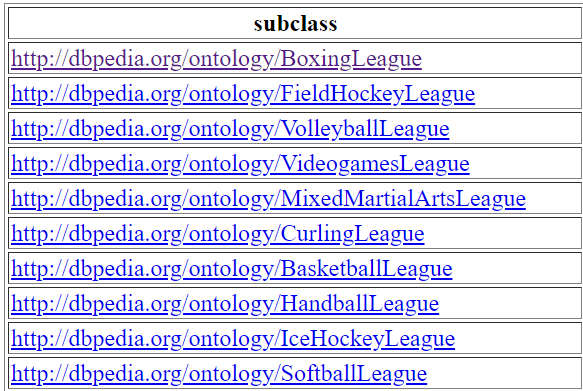
\includegraphics{Quest31}
            \end{center}
            \item \underline{Donner la liste des propriétés employées pour décrire les instances de la classe choisie.}
            \begin{verbatim}
PREFIX rdf: <http://www.w3.org/1999/02/22-rdf-syntax-ns#>
PREFIX owl: <http://www.w3.org/2002/07/owl#>
SELECT ?inst ?prop
WHERE {
?inst rdf:type <http://dbpedia.org/ontology/.....>.
?inst ?prop <http://dbpedia.org/ontology/......>
}
LIMIT 100
            \end{verbatim}
            \item \underline{Vérifier si ces propriétés ont des sous-propriétés.}
            \begin{verbatim}
PREFIX rdf: <http://www.w3.org/1999/02/22-rdf-syntax-ns#>
PREFIX owl: <http://www.w3.org/2002/07/owl#>
ASK
FROM <http://dbpedia.org/ontology/RacingDriver>
WHERE {
?inst rdf:type <http://dbpedia.org/ontology/......>.
?inst ?prop <http://dbpedia.org/ontology/..........>.
?subprop rdfs:subPropertyOf ?prop
}
            \end{verbatim}
        \end{enumerate}
    \end{justify}


    \section{Interrogation d'un flux RSS exporté en RDF:}
    \begin{justify}
        \begin{enumerate}
            \item \underline{Quels sont les titres des articles (rss:item) publiés dans le flux RSS ?}
            \begin{verbatim}
String req1 = "PREFIX vCard: <http://www.w3.org/2001/vcard-rdf/3.0#> "
                + "PREFIX rss: <http://purl.org/rss/1.0/> "
                + "PREFIX foaf: <http://xmlns.com/foaf/0.1/> "
                + "PREFIX rdf:<http://www.w3.org/1999/02/22-rdf-syntax-ns#>"
                + ""
                + "SELECT ?titre "
                + "FROM <http://www.w3.org/2001/sw/SW-FAQ-feed.rdf>"
                + " WHERE { "
                + " ?item rdf:type rss:item ."
                + " ?item rss:title ?titre"
                + "} ";
            \end{verbatim}
            \item \underline{Quel est le titre (rss:title) du flux (rss:channel) RSS ?}
            \begin{verbatim}
String req2 = "PREFIX vCard: <http://www.w3.org/2001/vcard-rdf/3.0#> "
                + "PREFIX rss: <http://purl.org/rss/1.0/> "
                + "PREFIX foaf: <http://xmlns.com/foaf/0.1/> "
                + "PREFIX rdf:<http://www.w3.org/1999/02/22-rdf-syntax-ns#>"
                + ""
                + "SELECT ?titre "
                + "FROM <http://www.w3.org/2001/sw/SW-FAQ-feed.rdf>"
                + " WHERE { "
                + " ?item rdf:type rss:channel ."
                + " ?item rss:title ?titre"
                + "} ";
            \end{verbatim}
            \item \underline{Donner les onze premiers articles du flux RSS par ordre chronologique.}
            \begin{verbatim}
String req3 = "PREFIX vCard: <http://www.w3.org/2001/vcard-rdf/3.0#> "
                + "PREFIX rss: <http://purl.org/rss/1.0/> "
                + "PREFIX foaf: <http://xmlns.com/foaf/0.1/> "
                + "PREFIX rdf:<http://www.w3.org/1999/02/22-rdf-syntax-ns#>"
                + ""
                + "SELECT ?article "
                + "FROM <http://www.w3.org/2001/sw/SW-FAQ-feed.rdf>"
                + " WHERE { "
                + " ?article rdf:type rss:item "
                + "} "
                + "LIMIT 11" ;
            \end{verbatim}
            \item \underline{Donner le deuxième article du flux RSS (ordre chronologique)}
            \begin{verbatim}
String req4 = "PREFIX vCard: <http://www.w3.org/2001/vcard-rdf/3.0#> "
                + "PREFIX rss: <http://purl.org/rss/1.0/> "
                + "PREFIX foaf: <http://xmlns.com/foaf/0.1/> "
                + "PREFIX rdf:<http://www.w3.org/1999/02/22-rdf-syntax-ns#>"
                + "" + "SELECT ?article "
                + "FROM <http://www.w3.org/2001/sw/SW-FAQ-feed.rdf>"
                + " WHERE { "
                + " ?article rdf:type rss:item "
                + "} "
                + "OFFSET 2"
                + "LIMIT 1";
            \end{verbatim}
            \item \underline{Donner l’avant dernier article du flux RSS (ordre chronologique)}
            \begin{verbatim}
String req5 = "PREFIX vCard: <http://www.w3.org/2001/vcard-rdf/3.0#> "
                + "PREFIX rss: <http://purl.org/rss/1.0/> "
                + "PREFIX foaf: <http://xmlns.com/foaf/0.1/> "
                + "PREFIX rdf:<http://www.w3.org/1999/02/22-rdf-syntax-ns#>"
                + ""
                + "SELECT ?article "
                + "FROM <http://www.w3.org/2001/sw/SW-FAQ-feed.rdf>"
                + " WHERE { "
                + " ?article rdf:type rss:item"
                + "} "
                + "OFFSET 51"
                + "LIMIT 51" ;
            \end{verbatim}
            \item \underline{Donner le deuxième ainsi que l’avant dernier article du flux RSS (requête UNION)}
            \begin{verbatim}
String req6 = "PREFIX vCard: <http://www.w3.org/2001/vcard-rdf/3.0#> "
                + "PREFIX rss: <http://purl.org/rss/1.0/> "
                + "PREFIX foaf: <http://xmlns.com/foaf/0.1/> "
                + "PREFIX rdf:<http://www.w3.org/1999/02/22-rdf-syntax-ns#>"
                + ""
                + "SELECT ?article "
                + "FROM <http://www.w3.org/2001/sw/SW-FAQ-feed.rdf>"
                + " WHERE { "
                + "{"
                + "SELECT ?article "
                + " WHERE { "
                + " ?article rdf:type rss:item"
                + "} "
                + "OFFSET 1"
                + "LIMIT 1"
                + "}"
                +"UNION"
                + "{"
                + "SELECT ?article "
                + " WHERE { "
                + " ?article rdf:type rss:item"
                + "} "
                + "OFFSET 51"
                + "LIMIT 51"
                + "}"
            \end{verbatim}
            \item \underline{Donner la liste des couples d’articles publiés à la même date}
            \begin{verbatim}
String req7 = "PREFIX vCard: <http://www.w3.org/2001/vcard-rdf/3.0#> "
                + "PREFIX rss: <http://purl.org/rss/1.0/> "
                + "PREFIX foaf: <http://xmlns.com/foaf/0.1/> "
                + "PREFIX rdf:<http://www.w3.org/1999/02/22-rdf-syntax-ns#>"
                + ""
                + "SELECT ?item ?titre ?date "
                + "FROM <http://www.w3.org/2001/sw/SW-FAQ-feed.rdf>"
                + " WHERE { "
                + " ?item rdf:type rss:item ."
                + " ?item rss:title ?titre ."
                + " ?item dc:date ?date"
                + "} ";
            \end{verbatim}
            \item \underline{Quels sont les articles publiés le 2007-04-12 ?}
            \begin{verbatim}
String req8 = "PREFIX vCard: <http://www.w3.org/2001/vcard-rdf/3.0#> "
                + "PREFIX rss: <http://purl.org/rss/1.0/> "
                + "PREFIX foaf: <http://xmlns.com/foaf/0.1/> "
                + "PREFIX rdf:<http://www.w3.org/1999/02/22-rdf-syntax-ns#>"
                + ""
                + "SELECT ?item ?titre ?date "
                + "FROM <http://www.w3.org/2001/sw/SW-FAQ-feed.rdf>"
                + " WHERE { "
                + " ?item rss:title ?titre ."
                + " ?item dc:date ?date"
                + "FILTER xsd:dateTime(?pub_date) "
                +">= \""20070412T00:00+00:00"^^xsd:string &&"
                + " xsd:dateTime(?pub_date) "
                +"< \""20070412T00:00+00:00"^^xsd:string"
                + "} ";
            \end{verbatim}
            \item \underline{Donnez la liste des auteurs (sans répétition) des articles dans ce flux RSS ?}
            \begin{verbatim}
String req9 = "PREFIX vCard: <http://www.w3.org/2001/vcard-rdf/3.0#> "
                + "PREFIX rss: <http://purl.org/rss/1.0/> "
                + "PREFIX foaf: <http://xmlns.com/foaf/0.1/> "
                + "PREFIX rdf:<http://www.w3.org/1999/02/22-rdf-syntax-ns#>"
                + ""
                + "SELECT "
                + "?item ?titre (distinct ?author) "
                + "FROM <http://www.w3.org/2001/sw/SW-FAQ-feed.rdf>"
                + " WHERE { "
                + " ?item rdf:type rss:item ."
                + " ?item rss:title ?titre ."
                + " ?item dc:author ?author"
                + "} ";
            \end{verbatim}
            \item  \underline{Dites si le flux RSS utilise la propri\'et\'e “title” d\'efinie par l\rq{espace} de nommage}\\ \underline{ Dublin Core (“dc:”)} \\
            \begin{verbatim}
String req10 = "PREFIX dc:<http://purl.org/dc/elements/1.1/>"
                +"PREFIX rdf: <http://www.w3.org/1999/02/22-rdf-syntax-ns#>"
                +" "
                +"SELECT ?f "
                +"FROM <http://www.w3.org/2001/sw/SW-FAQ-feed.rdf>"
                + " WHERE { "
                +"?f dc:title ?o"
                +" }";
            \end{verbatim}
            \item \underline{Dites si le flux RSS utilise la propriété “subject” définie par l’espace de nommage} \\ \underline{Dublin Core.}
            \begin{verbatim}
String req11 = "PREFIX dc:<http://purl.org/dc/elements/1.1/>"
                +"PREFIX rdf: <http://www.w3.org/1999/02/22-rdf-syntax-ns#>"
                +" "
                +"SELECT DISTINCT ?s "
                +"FROM <http://www.w3.org/2001/sw/SW-FAQ-feed.rdf>"
                + " WHERE { "
                +"?s dc:subject ?o "
                +" }"
                +"LIMIT 1";
            \end{verbatim}
            \item \underline{Donnez la liste des dates de publication de tous les articles du flux RSS.}
            \begin{verbatim}
String req12 = "PREFIX xsd: <http://www.w3.org/2001/XMLSchema#>"
                + " PREFIX dc: <http://purl.org/dc/elements/1.1/>"
                + " PREFIX rdf: <http://www.w3.org/1999/02/22-rdf-syntax-ns#>"
                + " PREFIX rss: <http://purl.org/rss/1.0/>"
                + "PREFIX swq: <http://www.w3.org/2001/sw/SW-FAQ#>"
                + "SELECT ?o"
                + " FROM <http://www.w3.org/2001/sw/SW-FAQ-feed.rdf>"
                + "WHERE { ?s dc:date ?o}";
            \end{verbatim}
        \end{enumerate}
    \end{justify}


    \section{Interrogation du réseau social de l'UE :}
    \begin{justify}
        \begin{enumerate}
            \item \underline{Est il vrai que GpersonalFriend $\subseteq$ GsocialFriend ?}
            \begin{verbatim}
PREFIX rdf: <http://www.w3.org/1999/02/22rdfsyntaxns#>
PREFIX foaf: <http://xmlns.com/foaf/0.1/> 
PREFIX ws: <http://www.lirmm.fr/˜ulliana/HMIN234.rdf#> 
PREFIX owl: <http://www.w3.org/2002/07/owl#>
 ASK
 FROM WHERE {
                GpersonalFriend ?inc GsocialFriend 
}

            \end{verbatim}
            \item \underline{Est il vrai que GsocialFriend $\subseteq$ GpersonalFriend ?}
            \begin{verbatim}
PREFIX rdf: <http://www.w3.org/1999/02/22rdfsyntaxns#>
PREFIX foaf: <http://xmlns.com/foaf/0.1/> 
PREFIX ws: <http://www.lirmm.fr/˜ulliana/HMIN234.rdf#> 
PREFIX owl: <http://www.w3.org/2002/07/owl#>
ASK
 FROM WHERE { 
GsocialFriend ?inc GpersonalFriend 
}
            \end{verbatim}
            \item \underline{Est il vrai que GpersonalFriend, GsocialFriend $\subseteq$ Gknows ?}
            \begin{verbatim}
PREFIX rdf: <http://www.w3.org/1999/02/22rdfsyntaxns#>
PREFIX foaf: <http://xmlns.com/foaf/0.1/>
PREFIX ws: <http://www.lirmm.fr/˜ulliana/HMIN234.rdf#>
PREFIX owl: <http://www.w3.org/2002/07/owl#>
ASK
FROM WHERE {
 WHERE {
 GpersonalFriend ?inc Gknows
}
UNION
WHERE {
 GsocialFriend ?inc Gknows
}
}

            \end{verbatim}
        \end{enumerate}
    \end{justify}
\end{document} 